\chapter{Campi conservativi e irrotazionali}

Affronteremo i successivi discorsi in $\R^3$

\section{Richiamo sui campi vettoriali}

Ricordiamo come un campo vettoriale in  sia una funzione del tipo
\begin{align}
	{}&\deffuncRgen{\vecF}{3}{3} \spacer A \text{ aperto}\\
	&\vecF\in C^0(A)
\end{align}

Abbiamo già definito il \textbf{lavoro di un campo vettoriale} come
\begin{align}
	W_{ab}= \int_{\gamma} ds \braket{F|T}= \int_{a}^{b} dt \sum_{i=1}^{3}F_i(x_1(t),x_2(t),x_3(t)) \cdot x'_i(t)
\end{align}

\section{Forme lineari}

Le forme lineari sono un modo alternativo per studiare i campi vettoriali. 

La forma $\omega$ associata al campo $\vecF$ si esprime come
\begin{align}
	\omega = F_1 dx + F_2 dy + F_3 dz
\end{align}

Per le forme lineari vale la proprietà di linearità:
\begin{align}
	{}&\omega_1 = \sum F_i dx_i \spacer \omega_2 = \sum G_i dx_i \spacer \alpha , \beta \in R\\
	&\omega = \alpha \omega_1 + \beta \omega_2 = \sum (\alpha F_i + \beta G_i)dx_i
\end{align}

Le forme lineari possono quindi essere anche viste come
\begin{align}
	\omega = \braket{F|dr}
\end{align}

E quindi si può esprimere il lavoro come
\begin{align}
	W_{ab}=\int_{\gamma} \omega
\end{align}
\newpage
E possiamo quindi riscrivere le proprietà come
\begin{enumerate}
	\item \textbf{Linearità}
	\begin{align}
		\int_\gamma \alpha \omega_1 + \beta \omega_2 =  \alpha \int_\gamma \omega_1 + \beta \int_\gamma \omega_2
	\end{align}
	\item \textbf{Additività sui cammini}
	\begin{align}
		\gamma = \gamma_1 \cup \gamma_2 \spacer \gamma_1 \cap \gamma_2 = \emptyset \implies  \int_\gamma \omega =  \int_{\gamma_1} \omega +  \int_{\gamma_2} \omega
	\end{align}
	\item \textbf{Curve analoghe}
	
	Date $\gamma_1$ e $\gamma_2$ equivalenti si avrà che 
	\begin{enumerate}
		\item con stesso orientamento 
		\begin{align}
			\int_{\gamma_1} \omega =  \int_{\gamma_2} \omega
		\end{align}
		\item con orientamento opposto
		\begin{align}
			\int_{\gamma_1} \omega =  -\int_{\gamma_2} \omega
		\end{align}
	\end{enumerate}
\end{enumerate}

Vediamo un paio di esempi.

\begin{figure}[!htb]
	\center{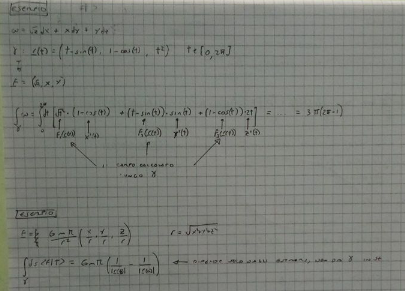
\includegraphics[width=\textwidth]
		{images/esCV1.png}
		\caption{\label{fig:my-label}}}
\end{figure}

\newpage

\section{Campi conservativi}

Il secondo esempio del paragrafo precedente ci spinge a farci una domanda: quando si ha che il lavoro di un campo vettoriale dipende solo dagli estremi del percorso?

Questo ci porta a dare la definizione di \textbf{campo conservativo}, ovvero un campo $\vecF$ tale che
\begin{align}
	\exists \deffuncRgen{U}{3}{} \spacecomma U\in C^1(A) \spacer \nabla U = \vecF
\end{align}

Con $U$ che prende il nome di \textbf{potenziale} di $\vecF$.

Nel linguaggio delle forme lineari si dice che è una forma $\omega$ è \textbf{esatta} se
\begin{align}
	\exists \; U \taleche \omega = \sum_{i=1}^{3} U_{x_i} dx_i
\end{align}

Ma quanti potenziali può ammettere $\vecF$ in un dominio $A\subset \R^3$ aperto?
\bigskip

Supponiamo di avere due potenziali $U,V$ per $\vecF$. Avremo che in $A$
\begin{align}
	\nabla U = \nabla V \implies \nabla (U-V)=\veczero \implies U-V = cost.
\end{align}

E che quindi tutti i potenziali in $A$ sono uguali a meno di una costante.

Ma in che modo ci sono utili questi potenziali? Lo scopriamo nel seguente \textbf{teorema:}

\bigskip

\textit{Sia $\vecF$ un campo conservativo dotato di potenziale $U$ e sia $\gamma$ curva di estremi $\vecP_i$ e $\vecP_f$, avremo che}
\begin{align}
	\int_{\gamma} ds \braket{F|T}= U(\vecP_f) - U(\vecP_i)
\end{align} 

\bigskip

Per la dimostrazione si procede notando che
\begin{align}
	\dertot{}{t}U(x_1(t) , x_2(t) , x_3(t)) = \sum_{i=1}^{3} U_{x_i} x'_i(t)= \sum_{i=1}^{3} F_i x'_i(t)
\end{align}

E quindi sostituendo nell'integrale del lavoro otteniamo, avendo definito $\vecP_i = \underline{r}(a)$ e $\vecP_f = \underline{r}(b)$
\begin{align}
	\int_{\gamma} ds \braket{F|T} {}&= \int_{a}^{b} dt \sum_{i=1}^{3}F_i(x_1(t),x_2(t),x_3(t)) \cdot x'_i(t) = \continue &=\int_{a}^{b} dt \dertot{}{t}U(x_1(t) , x_2(t) , x_3(t)) = U(\vecP_f) - U(\vecP_i)
\end{align}

\subsection{Caratterizzazione dei campi conservativi}

Sia un dominio $A\subset \R^3$ aperto e connesso, e sia un campo vettoriale $\vecF \in C^0(A)$. Avremo che le tre seguenti affermazioni sono equivalenti:
\begin{enumerate}
	\item $\vecF$ è conservativo
	\item $\oint_\gamma ds \braket{F|T}=0 \quad \forall \gamma \text{ chiusa } \subset A$
	\item $\int_{\gamma_1}ds \braket{F|T} = \int_{\gamma_2}ds \braket{F|T}$ date due curve $\gamma_1 \spacecomma \gamma_2$ con stessi estremi ed orientamento
\end{enumerate}

Vediamo come la 1 implichi la 2, dato che utilizzando il teorema dei potenziali e prendendo $\vecP_f=\vecP_i$ otteniamo un integrale chiuso il risultato è nullo.

\bigskip

A sua volta la 2 implica la 3, dato che se due curve hanno gli stessi estremi si avrà che
\begin{figure}[!htb]
	\center{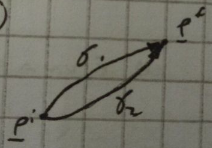
\includegraphics[width=0.3\textwidth]
		{images/cequiv.png}
		\caption{\label{fig:my-label}}}
\end{figure}
\begin{align}
	{}&\gamma = \gamma_1 \cup (-\gamma_2) \text{ curva chiusa}\\
	&\oint_\gamma = \int_{\gamma_1} + \int_{-\gamma_2} = \int_{\gamma_1} - \int_{\gamma_2} \nextpassage
	& \oint_\gamma =0 \implies \int_{\gamma_1} - \int_{\gamma_2} = 0 \implies \int_{\gamma_1} = \int_{\gamma_2}
\end{align}

\newpage

Infine la 3 implica la 1. Fissato $\vecP^0\in A$ e definita $\Gamma(\vecP) = \gamma_{\vecP^0 \rightarrow\vecP}\subset A$

Dimostriamo come dato 
\begin{align}
	\int_{\Gamma(\vecP)} ds \braket{F|T}=U(\vecP)
\end{align}
$U(\vecP)$ sia un potenziale.

Ci chiediamo
\begin{align}
	\limit{h}{0} \frac{U(x+h,y,z) - U(x,y,z)}{h} \doubteq F_1
\end{align}

Iniziamo scomponendo $\Gamma(\vecP^h)$ nel seguente modo
\begin{figure}[!htb]
	\center{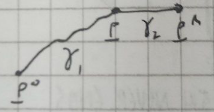
\includegraphics[width=0.3\textwidth]
		{images/cscomp.png}
		\caption{\label{fig:my-label}}}
\end{figure}

\begin{align}
	U(x+h,y,z) = \int_{\Gamma(\vecP^h)} ds \braket{F|T} = \int_{\gamma_1} ds \braket{F|T} + \int_{\gamma_2} ds \braket{F|T}
\end{align}

Il primo integrale è semplicemente $U(x,y,z)$, mentre la curva $\gamma_2$ può essere parametrizzata nel seguente modo
\begin{align}
	\underline{r}(t)= \triple{x(t)=t}{y(t)=y}{z(t)=z} \quad t\in[x,x+h]
\end{align}
Otteniamo così
\begin{align}
	U(x+h,y,z) {}&= U(x,y,z) + \int_{x}^{x+h} dt \; [F_1(x,y,z) \cdot 1 + F_2 \cdot 0 + F_3 \cdot 0]= \continue
	&= U(x,y,z) + \int_{x}^{x+h} dt \; F_1(x,y,z)
\end{align}
Sostituendo nel rapporto incrementale otteniamo
\begin{align}
	U_x(x,y,z) {}&= \limit{h}{0} \fracn{h} \left(  \cancel{U(x,y,z)}  + \int_{x}^{x+h} dt \; F_1(x,y,z) - \cancel{U(x,y,z)} \right) = \continue
	&= \limit{h}{0} \fracn{h} \int_{x}^{x+h} dt \; F_1(x,y,z) = \limit{h}{0} \fracn{h} F_1(x,y,z) \int_{x}^{x+h} dt = \continue
	&= \limit{h}{0} \fracn{h} F_1(x,y,z) h = F_1(x,y,z)
\end{align}
In modo analogo si dimostrano le altre due componenti, e abbiamo così dimostrato che $U(x,y,z)$ è un potenziale, e che quindi $\vecF$ è un campo conservativo. E che per un campo conservativo non importa il tragitto, ma solo gli estremi, dato che $\Gamma(\vecP^h)$ poteva essere parametrizzata in diversi modi ottenendo sempre lo stesso risultato.

\bigskip

Ci chiediamo però: operativamente, come riconosciamo quanto un campo è conservativo? Entra in gioco il \textbf{rotore} del campo $\vecF$:
\begin{align}
	rot \vecF {}&= curl \vecF = \nabla \times \vecF = \det \matrixThreeThree{\hat{i}}{\hat{j}}{\hat{k}}{\partialder{}{x}}{\partialder{}{y}}{\partialder{}{z}}{F_1}{F_2}{F_3}= \continue
	&= \hat{i} \left( \partialder{F_3}{y} - \partialder{F_2}{z} \right)  + \hat{j}  \left( \partialder{F_1}{z} - \partialder{F_3}{x} \right) + \hat{k} \left( \partialder{F_2}{x} - \partialder{F_1}{y} \right)
\end{align}

La matrice è detta \textbf{simbolica} e il determinante è detto \textbf{formale}, perché non rappresentano quantità esistenti ben definite, ma solo "concetti".



Notiamo come se una delle componenti del campo è nulla, e quindi ci troviamo su un piano, il rotore si ridurrà ad una sola componente.

\bigskip

Introduciamo quindi il concetto di \textbf{campo irrotazionale}, ovvero di campo con rotore nullo
\begin{align}
	\nabla \times \vecF = \veczero
\end{align}

Una forma differenziale associata ad un campo irrotazionale viene detta \textbf{chiusa}.

E possiamo quindi dare la \textbf{condizione necessaria di conservatività}:

\bigskip

\textit{Se un campo $\vecF\in C^1(A)$ è conservativo,allora è anche irrotazionale.}

\bigskip

La dimostrazione si appoggia al teorema di Schwartz sulle derivate miste. Infatti essendo $U_{x_i x_j}=U_{x_j x_i}$ si ha che
\begin{align}
	\partialder{F_i}{x_j} = \partialder{F_j}{x_i} \implies \partialder{F_i}{x_j} - \partialder{F_j}{x_i} =0 \quad \forall i,j \implies \nabla \times \vecF=\veczero
\end{align}

\begin{figure}[!htb]
	\center{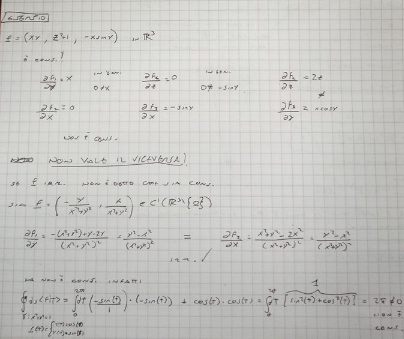
\includegraphics[width=\textwidth]
		{images/cirr.png}
		\caption{\label{fig:my-label}}}
\end{figure}

\newpage

\section{Domini semplicemente connessi}

Sia $A\subset \R^3$ un dominio aperto e connesso. Avremo che se ogni curva $\gamma\subset A$ chiusa, regolare/a tratti e semplice è frontiera di un insieme $D\subset A$ allora si dice che $A$ è \textbf{semplicemente connesso}.

In altre parole un dominio $A$ è s.c. se ogni $\gamma\subset A$ può essere ridotta con continuità ad un punto senza uscire da $A$.

In $\R^2$ questo significa che un dominio s.c. non ammette buchi al suo interno; cosa che invece cambia per $n\geq 3$, dove se il buco è di un singolo punto il dominio è comunque s.c.

\bigskip

Esempi di insiemi s.c. sono tutti gli insiemi convessi, $\R^2$ e campi circolari, mentre non sono s.c. corone circolari $\R^2 \except{(x_0,y_0)}$ o $\R^3\except{\text{una retta}}$.

\bigskip

I domini semplicemente connessi sono molto comodi da studiare, in quanto portano con loro diversi teoremi utili:

\begin{enumerate}
	\item \textbf{S.C. e convessità}
	
	\textit{Sia $\vecF$ un campo irrotazionale in $A\subset \R^3$}
	
	\textit{Allora se $A$ è s.c. segue che $\vecF$ è convesso in $A$.}
	
	La dimostrazione viene rimandata a quando studieremo il th. di Stokes, in quanto semplifica notevolmente lo studio.
	
	
	\item \textbf{S.C. e conservatività locale}
	
	\textit{Se un campo $\vecF$ è irrotazionale in un dominio aperto $A\subset\R^{2,3}$, allora è anche localmente conservativo in $A$ .}
	
	Avremo quindi dei potenziali \textbf{locali} e che $\exists I(\vecP^0 \in A) \taleche \text{ se } I(\vecP^0) \text{ s.c. } \implies \vecF \text{ cons. }$ e che $I(\vecP^0)=B(\vecP^0,r)$.
	
	\item \textbf{S.C. e conservatività nel piano}	
	
	\textit{Dato un campo vettoriale $\vecF=(F_1(x,y),F_2(x,y))$, se per $(x,y)\in A\subset \R^2$ si ha che $F_{1_x}=F_{2_y}$ allora $\vecF$ è conservativo.}
	
	Diamo in questo caso una dimostrazione del teorema più restrittiva nel prossimo paragrafo, giusto per darci un'idea su come si costruiscano i potenziali.
\end{enumerate}

\newpage

\section{Lemma di Poincarré}

Prima di procedere diamo una definizione utile ai fini di una del seguente teorema:

Un dominio si dice \textbf{stellato rispetto al punto $\vecx^0$} se ogni ogni punto del dominio è collegabile a $\vecx^0$ tramite un segmento.

\textbf{Nota:} un insieme convesso è stellato rispetto ad ogni suo punto. 

\textbf{Nota:} Un dominio stellato è anche s.c., ma un dominio s.c. non è detto sia stellato (e.x. domini a "ferro di cavallo").

\bigskip

Diamo ora il \textbf{Lemma di Poincarré}, il quale ci dice che

\bigskip

\textit{Sia $\vecF$ irrotazionale in un dominio $A$ stellato rispetto ad un punto $\vecP^0$, allora $\vecF$ è anche conservativo.}

\bigskip

Diamo del lemma una dimostrazione costruttiva, ovvero dimostriamo il lemma costruendo un potenziale, e per semplicità ci poniamo in $\R^2$ con $\vecP^0=(0,0)$.

Sia $\gamma=s_{\vecP^0 \rightarrow\vecP}$ il segmento che unisce i punti a $(0,0)$, avremo che
\begin{align}
	\gamma \taleche \underline{r}(t)=\double{x(t)=tx}{y(t)=ty} \quad t\in[0,1]
\end{align}
E dato
\begin{align}
	U(x,y)= \int_{\gamma} ds \braket{F|T}= \int_{0}^{1} dt [F_1(tx,ty) \cdot x + F_2(tx,ty) \cdot y]
\end{align}
Dobbiamo dimostrare che
\begin{align}
	U_x=F_1 \spacer U_y=F_2
\end{align}

Per farlo commettiamo un "abuso" e utilizziamo una nozione, lo scambio tra derivata e integrale, che ancora non sappiamo dimostrare:
\begin{align}
	\partialder{U}{x}{}&= \partialder{}{x} \int_{0}^{1} dt [F_1(tx,ty) \cdot x + F_2(tx,ty) \cdot y] = \continue
	&=\int_{0}^{1} dt \left[\partialder{}{x}(F_1(tx,ty) \cdot x) + \partialder{}{x}(F_2(tx,ty) \cdot y)\right]= \continue
	&= \int_{0}^{1} dt \left[  F_1(tx,ty) + (F_{1_x}(tx,ty)\cdot t)\cdot x +  (F_{2_x}(tx,ty)\cdot t)\cdot y  \right]= \continue
	&= \int_{0}^{1} dt \left[  F_1(tx,ty) + t(F_{1_x}(tx,ty)\cdot x + F_{2_x}(tx,ty)\cdot y)  \right]
\end{align}
Facciamo ora uso dell'irrotazionalità di $\vecF$ e integrando per parti otteniamo
\begin{align}
	\partialder{U}{x}{}&= \int_{0}^{1} dt \left[  F_1(tx,ty) + t(F_{1_x}(tx,ty)\cdot x + F_{2_x}(tx,ty)\cdot y)  \right]= \continue
	&= \int_{0}^{1} dt \left[  F_1(tx,ty) +  \dertot{}{t}F_1(tx,ty)   \right] =\continue
	&= \int_{0}^{1} dt   F_1(tx,ty) +  \int_{0}^{1} dt  \dertot{}{t}F_1(tx,ty) =  \continue
	&= \cancel{\int_{0}^{1} dt F_1(tx,ty)} + tF_1(tx,ty)|_{t=0}^{t=1} - \cancel{\int_{0}^{1} dt F_1(tx,ty)}= \continue
	&= F_1(x,y)
\end{align}
Che è ciò che volevamo. In modo identico si dimostra $U_y= F_2$.

\bigskip

Abbiamo così un pratico criterio per studiare la conservatività di un campo in un dominio:
\begin{enumerate}
	\item $\nabla \times \vecF \doubteq \veczero$
	\item $A$ è s.c. o stellato?
\end{enumerate}

Se la risposta è positiva ad entrambe le domande il campo è conservativo nel dominio $A$.
